\chapter{Results} \label{sec:results}
\epigraph{We must be clear that when it comes to atoms, language can be used only as in poetry.}{Niels Bohr}
\begin{figure}[H]
	\centering
	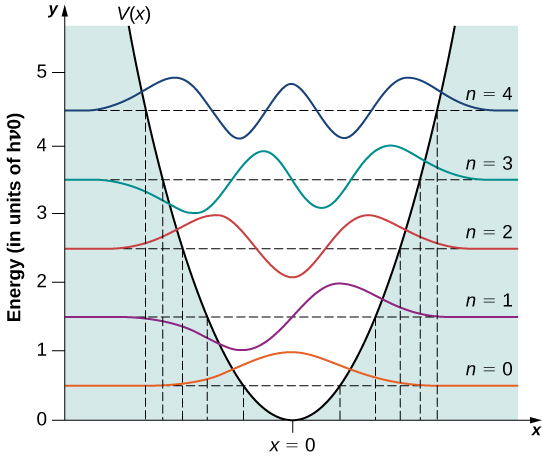
\includegraphics[scale=0.9]{Images/qho.jpg}
	\caption{The quantum harmonic oscillator, with the Hermite functions represented up to 4th order. As in classical mechanics, the harmonic oscillator can describe various quantum systems, such as lattice vibration (phonons) and quantum fields.}
\end{figure}

\section{Ground state energies}
\subsection{Quantum Dots}
\subsubsection{Without interaction}
We will start studying systems with no interaction between particles. The number of closed-shell particles are given by \eqref{eq:HOclosedshell} and the exact energies are found from formula \eqref{eq:HOenergies}. The first 5 closed-shell energies for $\omega=1$ are presented in table \eqref{tab:nointeractionHO2D} and \eqref{tab:nointeractionHO3D} for two and three dimensions respectively.
\begin{table} [H]
	\caption{2D  \vspace{2mm}}
	\begin{tabularx}{\textwidth}{X|X:X:X} \hline\hline
		\label{tab:nointeractionHO2D}
		N & Obtained energy & Variance & Exact energy \\ \hline
		2 & 2.0 & 0.0 & 2\\ 
		6 & 10.0 & 0.0 & 10\\
		12 & 28.0 & 0.0 & 28 \\
		20 & 60.0 & 0.0 & 60 \\
		30 & 110.0 & 0.0 & 110 \\ \hline\hline
	\end{tabularx}
\end{table}

\begin{table} [H]
	\caption{3D  \vspace{2mm}}
	\begin{tabularx}{\textwidth}{X|X:X:X} \hline\hline
		\label{tab:nointeractionHO3D}
		N & Obtained energy & Variance & Exact energy \\ \hline
		2 & 3.0 & 0.0 & 3\\ 
		8 & 18.0 & 0.0 & 18\\
		20 & 54.0 & 0.0 & 54 \\
		40 & 134.0 & 0.0 & 134 \\
		70 & 299.0 & 0.0 & 299 \\ \hline\hline
	\end{tabularx}
\end{table}

\subsubsection{With interaction}


\section{Comparison of Wave Functions}
Compare machine learning wave functions to standard VMC wave functions